\begin{table}[ht!]
    \centering
    \resizebox{15cm}{!} {
    \begin{tabular}{|l|l|}
    \hline
         \textbf{CU-39}     &  \textbf{Tarjeta de los ingresos en 7 días} \\ \hline
         \textbf{Requisitos relacionados}       & RF-5, RF-5.6 \\ \hline
         \textbf{Descripción}    & Debe proporcionar el número de los ingresos en 7 días \\& en función del filtrado aplicado, excepto el filtro fecha, \\& ya que cogerá un intervalo de 7 días desde la fecha de \\& actualización de la hoja. \\ \hline   
         \textbf{Precondiciones}      &  Haber accedido a la hoja de ingresos y altas \\& hospitalarias.\\ \hline
         \textbf{Acciones}      &  \parbox[p][0.35\textwidth][c]{10cm}{
            \begin{enumerate}\tightlist
                  \item Se recoge de la base de datos la suma de los ingresos confirmados de la tabla hospitales, aplicando los filtros de la hoja ingresos y altas hospitalarias, excepto el filtro fecha, el cual es ignorado y se pone por filtro de fecha 7 días desde la fecha de actualización de la hoja.
                 \item Se muestra en la tarjeta el resultado del paso anterior.
            \end{enumerate}} \\ \hline
         \textbf{Postcondiciones}       & -\\ \hline
         \textbf{Excepciones}       & - \\ \hline
         \textbf{Importancia}   & Alta. \\
         \hline
    \end{tabular}}
    \caption{CU-39 - Tarjeta de los ingresos en 7 días}
    \label{tab:my_label}
\end{table}

\begin{table}[ht!]
    \centering
    \resizebox{15cm}{!} {
    \begin{tabular}{|l|l|}
    \hline
         \textbf{CU-40}     &  \textbf{Tarjeta de las altas en 7 días} \\ \hline
         \textbf{Requisitos relacionados}       & RF-5, RF-5.7 \\ \hline
         \textbf{Descripción}    & Debe proporcionar el número de altas en 7 días en función\\& del filtrado aplicado, excepto el filtro fecha, ya que cogerá \\& un intervalo de 7 días desde la fecha de actualización de \\& la hoja. \\ \hline   
         \textbf{Precondiciones}      & Haber accedido a la hoja de ingresos y altas hospitalarias. \\ \hline
         \textbf{Acciones}      &  \parbox[p][0.3\textwidth][c]{10cm}{
            \begin{enumerate}\tightlist
                \item Se recoge de la base de datos la suma de las altas confirmadas de la tabla hospitales, aplicando los filtros de la hoja ingresos y altas hospitalarias, excepto el filtro fecha, el cual es ignorado y se pone por filtro de fecha 7 días desde la fecha de actualización de la hoja.
                 \item Se muestra en la tarjeta el resultado del paso.
            \end{enumerate}} \\ \hline
         \textbf{Postcondiciones}       & -\\ \hline
         \textbf{Excepciones}       & - \\ \hline
         \textbf{Importancia}   & Alta. \\
         \hline
    \end{tabular}}
    \caption{CU-40 - Tarjeta de los ingresos en 7 días}
    \label{tab:my_label}
\end{table}

\begin{table}[ht!]
    \centering
    \resizebox{15cm}{!} {
    \begin{tabular}{|l|l|}
    \hline
         \textbf{CU-41}     &  \textbf{\makecell{Gráfico de evolución diaria de ingresos por tipo de\\ hospitalización}} \\ \hline
         \textbf{Requisitos relacionados}       & RF-5, RF-5.8 \\ \hline
         \textbf{Descripción}    & Debe mostrar un gráfico de barras 100\% apiladas \\& verticalmente con la evolución diaria del porcentaje de \\& hospitalizaciones UCI y hospitalizaciones convencionales, \\&en función del filtrado aplicado. \\ \hline   
         \textbf{Precondiciones}      & Haber accedido a la hoja de ingresos y altas hospitalarias. \\ \hline
         \textbf{Acciones}      &  \parbox[p][0.4\textwidth][c]{10cm}{
            \begin{enumerate}\tightlist
                 \item Se recoge de la base de datos la suma de los ingresos de la tabla hospitales, aplicando los filtros que de la hoja ingresos y altas hospitalarias.
                 \item Se dividen visualmente por el tipo de hospitalización y se calcula que porcentaje del total corresponde a cada tipo.
                 \item Se muestra el grafico de barras 100\% apiladas verticalmente con los datos del apartado anterior distribuidos sobre el eje y que contiene las fechas en granularidad diaria.
            \end{enumerate}} \\ \hline
         \textbf{Postcondiciones}       & - \\ \hline
         \textbf{Excepciones}       & - \\ \hline
         \textbf{Importancia}   & Alta. \\
         \hline
    \end{tabular}}
    \caption{CU-41 -  Gráfico de evolución diaria de ingresos por tipo
de hospitalización.}
    \label{tab:my_label}
\end{table}
\begin{table}[ht!]
    \centering
    \resizebox{15cm}{!} {
    \begin{tabular}{|l|l|}
    \hline
         \textbf{CU-42}     &  \textbf{Gráfico de evolución diaria de altas e ingresos} \\ \hline
         \textbf{Requisitos relacionados}       & RF-5, RF-5.9 \\ \hline
         \textbf{Descripción}    & Debe mostrar un gráfico de columnas agrupadas y de \\&líneas con la evolución diaria de altas e ingresos. \\ \hline
         \textbf{Precondiciones}      & Haber accedido a la hoja de ingresos y altas hospitalarias. \\ \hline
         \textbf{Acciones}      &  \parbox[p][0.45\textwidth][c]{10cm}{
            \begin{enumerate}\tightlist
                 \item Se recoge de la base de datos la suma de las altas de la tabla hospitales, aplicando los filtros que de la hoja ingresos y altas hospitalarias.
                 \item Se recoge de la base de datos la suma de los ingresos de la tabla hospitales, aplicando los filtros que de la hoja ingresos y altas hospitalarias.
                 \item Se muestra el grafico de columnas agrupadas y de líneas con los datos calculados en los apartados anteriores distribuidos sobre el eje y que contiene las fechas en granularidad diaria.
            \end{enumerate}} \\ \hline
         \textbf{Postcondiciones}       & - \\ \hline
         \textbf{Excepciones}       & - \\ \hline
         \textbf{Importancia}   & Alta. \\
         \hline
    \end{tabular}}
    \caption{CU-42 - Gráfico de evolución diaria de altas e ingresos.}
    \label{tab:my_label}
\end{table}
\begin{table}[ht!]
    \centering
    \resizebox{15cm}{!} {
    \begin{tabular}{|l|l|}
    \hline
         \textbf{CU-43}     &  \textbf{\makecell{Gráfico de tasa de ingresos e ingresos UCI en 7\\ días cada 100.000 habitantes por comunidad}} \\ \hline
         \textbf{Requisitos relacionados}       & RF-5, RF-5.10 \\ \hline
         \textbf{Descripción}    &  Debe mostrar un gráfico de dispersión con ingresos\\& e ingresos UCI en 7 días cada 100.000 habitantes\\& agrupados por comunidad autónoma. \\ \hline  
         \textbf{Precondiciones}      & Haber accedido a la hoja de ingresos y altas hospitalarias. \\ \hline
         \textbf{Acciones}      &  \parbox[p][1.0\textwidth][c]{10cm}{
            \begin{enumerate}\tightlist
                 \item Se recoge de la base de datos, siguiendo una función programada en DAX, la suma de los ingresos de los últimos 7 días de la tabla hospitales, desde la fecha de tasa nuevos ingresos, y aplicando los filtros de la hoja de ingresos y altas hospitalarias.
                 \item Se recoge de la base de datos, siguiendo una función programada en DAX, la suma de los ingresos UCI de los últimos 7 días de la tabla hospitales, desde la fecha de tasa nuevos ingresos, y aplicando los filtros de la hoja de ingresos y altas hospitalarias.
                 \item Se recoge de la base de datos, la suma de la población de la tabla población, aplicando los filtros de la hoja de casos y muertes.
                 \item Se realiza la división de la suma de ingresos de los últimos 7 días calculada en el primer paso entre la suma de la población del tercer paso.
                 \item Se realiza la división de la suma de ingresos UCI de los últimos 7 días calculada en el segundo paso entre la suma de la población del tercer paso y se multiplica por 100.000.
                 \item Se agrupan tanto los datos obtenidos en el cuarto paso, como en el quinto paso por comunidad autónoma.
                 \item Se muestra el grafico de dispersión resultante con los datos calculados en el apartado anterior.         
            \end{enumerate}} \\ \hline
         \textbf{Postcondiciones}       & - \\ \hline
         \textbf{Excepciones}       & - \\ \hline
         \textbf{Importancia}   & Alta. \\
         \hline
    \end{tabular}}
    \caption{CU-43 - Gráfico de tasa de ingresos e ingresos UCI en 7 días cada 100.000 habitantes por comunidad.}
    \label{tab:my_label}
\end{table}

\begin{table}[ht!]
    \centering
    \resizebox{15cm}{!} {
    \begin{tabular}{|l|l|}
    \hline
         \textbf{CU-44}     &  \textbf{\makecell{Mapa de tasa de ingresos UCI en 7 días cada
\\ 100.000 habitantes}} \\ \hline
         \textbf{Requisitos relacionados}       & RF-5, RF-5.11 \\ \hline
         \textbf{Descripción}    & Debe mostrar un mapa coroplético con la tasa de ingresos UCI en \\&7 días cada 100.000 habitantes agrupado por comunidad autónoma. \\ \hline   
         \textbf{Precondiciones}      & Haber accedido a la hoja de ingresos y altas hospitalarias. \\ \hline
         \textbf{Acciones}      &  \parbox[p][0.55\textwidth][c]{12cm}{
            \begin{enumerate}\tightlist
                 \item Se recoge de la base de datos, siguiendo una función programada en DAX, la suma de los ingresos UCI de los últimos 7 días de la tabla hospitales, desde la fecha de tasa nuevos ingresos, y aplicando los filtros de la hoja de ingresos y altas hospitalarias.
                 \item Se recoge de la base de datos, la suma de la población de la tabla población, aplicando los filtros de la hoja de casos y muertes.
                 \item Se realiza la división de la suma de ingresos UCI de los últimos 7 días calculada en el primer paso entre la suma de la población del segundo paso y se multiplica por 100.000.
                 \item Se agrupa por comunidades autónomas.
                 \item Se muestra el mapa coroplético resultante.
            \end{enumerate}} \\ \hline
         \textbf{Postcondiciones}       & - \\ \hline
         \textbf{Excepciones}       & - \\ \hline
         \textbf{Importancia}   & Alta. \\
         \hline
    \end{tabular}}
    \caption{CU-44 - Mapa de tasa de ingresos UCI en 7 días cada
100.000 habitantes.}
    \label{tab:my_label}
\end{table}
\begin{table}[ht!]
    \centering
    \resizebox{15cm}{!} {
    \begin{tabular}{|l|l|}
    \hline
         \textbf{CU-45}     &  \textbf{\makecell{Mapa de tasa de ingresos en 7 días cada 100.000 \\ habitantes}} \\ \hline
         \textbf{Requisitos relacionados}       & RF-5, RF-5.12 \\ \hline
         \textbf{Descripción}    & Debe mostrar un mapa coroplético con la tasa de ingresos en 7 \\&días cada 100.000 habitantes agrupado por comunidad autónoma. \\ \hline   
         \textbf{Precondiciones}      & Haber accedido a la hoja de ingresos y altas hospitalarias. \\ \hline
         \textbf{Acciones}      &  \parbox[p][0.55\textwidth][c]{12cm}{
            \begin{enumerate}\tightlist
                 \item Se recoge de la base de datos, siguiendo una función programada en DAX, la suma de los ingresos de los últimos 7 días de la tabla hospitales, desde la fecha de tasa nuevos ingresos, y aplicando los filtros de la hoja de ingresos y altas hospitalarias.
                 \item Se recoge de la base de datos, la suma de la población de la tabla población, aplicando los filtros de la hoja de casos y muertes.
                 \item Se realiza la división de la suma de ingresos de los últimos 7 días calculada en el primer paso entre la suma de la población del segundo paso y se multiplica por 100.000.
                 \item Se agrupa por comunidades autónomas.
                 \item Se muestra el mapa coroplético resultante.
            \end{enumerate}} \\ \hline
         \textbf{Postcondiciones}       & - \\ \hline
         \textbf{Excepciones}       & - \\ \hline
         \textbf{Importancia}   & Alta. \\
         \hline
    \end{tabular}}
    \caption{CU-45 - Mapa de tasa de ingresos en 7 días cada 100
000 habitantes.}
    \label{tab:my_label}
\end{table}
\begin{table}[ht!]
    \centering
    \resizebox{15cm}{!} {
    \begin{tabular}{|l|l|}
    \hline
         \textbf{CU-46}     &  \textbf{Mostrar página de camas hospitalarias} \\ \hline
         \textbf{Requisitos relacionados}       & RF-6 \\ \hline
         \textbf{Descripción}    & Permite al usuario visualizar la página que contiene el \\&análisis de la ocupación de las camas hospitalarias. \\ \hline   
         \textbf{Precondiciones}      & Haber accedido al informe. \\ \hline
         \textbf{Acciones}      & Clickar en la pestaña de camas hospitalarias. \\ \hline
         \textbf{Postcondiciones}       & Has accedido a la hoja camas hospitalarias. \\ \hline
         \textbf{Excepciones}       & - \\ \hline
         \textbf{Importancia}   & Alta. \\
         \hline
    \end{tabular}}
    \caption{CU-46 - Mostrar página de camas hospitalarias.}
    \label{tab:my_label}
\end{table}
\begin{table}[ht!]
    \centering
    \resizebox{15cm}{!} {
    \begin{tabular}{|l|l|}
    \hline
         \textbf{CU-47}     &  \textbf{\makecell{Tarjeta de fecha de ocupación de camas \\ hospitalarias}} \\ \hline
         \textbf{Requisitos relacionados}       & RF-6, RF-6.5 \\ \hline
         \textbf{Descripción}    & Debe proporcionar la fecha de ocupación de camas \\& hospitalarias que se está aplicando a los gráficos de \\& la página, esta fecha va en función del filtro fecha. \\ \hline   
         \textbf{Precondiciones}      & Haber accedido a una hoja con esta tarjeta. \\ \hline
         \textbf{Acciones}      &  \parbox[p][0.2\textwidth][c]{10cm}{
            \begin{enumerate}\tightlist
                 \item Se recoge de la base de datos el resultado de la fecha más actual la tabla hospitales, aplicando antes el filtro de fecha.
                 \item Se muestra en la tarjeta la fecha recogida en el paso anterior.
            \end{enumerate}} \\ \hline
         \textbf{Postcondiciones}       & - \\ \hline
         \textbf{Excepciones}       & - \\ \hline
         \textbf{Importancia}   & Alta. \\
         \hline
    \end{tabular}}
    \caption{CU-47 - Tarjeta de fecha de ocupación de camas hospi-
talarias.}
    \label{tab:my_label}
\end{table}

\begin{table}[ht!]
    \centering
    \resizebox{15cm}{!} {
    \begin{tabular}{|l|l|}
    \hline
         \textbf{CU-48}     &  \textbf{\makecell{Tarjeta de porcentaje de camas ocupadas por \\ covid}} \\ \hline
         \textbf{Requisitos relacionados}       & RF-6, RF-6.6 \\ \hline
         \textbf{Descripción}    & Debe proporcionar el porcentaje de camas ocupadas por \\&covid en función del filtrado aplicado, excepto el filtro \\& fecha, el cual es ignorado y se pone por filtro de fecha \\& la fecha de actualización de la hoja. \\ \hline   
         \textbf{Precondiciones}      & Haber accedido a la hoja de camas hospitalarias. \\ \hline
         \textbf{Acciones}      &  \parbox[p][0.65\textwidth][c]{10cm}{
            \begin{enumerate}\tightlist
                 \item Se recoge de la base de datos las camas ocupadas por covid de la tabla hospitales, aplicando los filtros que de la hoja camas hospitalaria, excepto el filtro fecha, el cual es ignorado y se pone por filtro de fecha la fecha de actualización de la hoja.
                 \item Se recoge de la base de datos las camas totales de la tabla hospitales, aplicando los filtros que de la hoja camas hospitalarias, excepto el filtro fecha, el cual es ignorado y se pone por filtro de fecha la fecha de actualización de la hoja.
                 \item Se realiza la división de la suma de las camas ocupadas por covid calculada en el primer paso entre la suma de las camas totales del segundo paso y se multiplica por 100.
                 \item Se muestra en la tarjeta el resultado del paso anterior.
            \end{enumerate}} \\ \hline
         \textbf{Postcondiciones}       & - \\ \hline
         \textbf{Excepciones}       & - \\ \hline
         \textbf{Importancia}   & Alta. \\
         \hline
    \end{tabular}}
    \caption{CU-48 - Tarjeta de porcentaje de camas ocupadas por
covid.}
    \label{tab:my_label}
\end{table}
\begin{table}[ht!]
    \centering
    \resizebox{15cm}{!} {
    \begin{tabular}{|l|l|}
    \hline
         \textbf{CU-49}     &  \textbf{\makecell{Tarjeta de porcentaje de camas UCI ocupadas por \\ covid}} \\ \hline
         \textbf{Requisitos relacionados}       & RF-6, RF-6.7 \\ \hline
         \textbf{Descripción}    & Debe proporcionar el porcentaje de camas UCI ocupadas \\&por covid en función del filtrado aplicado excepto el filtro \\& fecha, el cual es ignorado y se pone por filtro de fecha la \\& fecha de actualización de la hoja. \\ \hline   
         \textbf{Precondiciones}      & Haber accedido a la hoja de camas hospitalarias. \\ \hline
         \textbf{Acciones}      &  \parbox[p][0.65\textwidth][c]{10cm}{
            \begin{enumerate}\tightlist
                 \item Se recoge de la base de datos las camas UCI ocupadas por covid de la tabla hospitales, aplicando los filtros que de la hoja camas hospitalaria, excepto el filtro fecha, el cual es ignorado y se pone por filtro de fecha la fecha de actualización de la hoja.
                 \item Se recoge de la base de datos las camas UCI totales de la tabla hospitales, aplicando los filtros que de la hoja camas hospitalarias, excepto el filtro fecha, el cual es ignorado y se pone por filtro de fecha la fecha de actualización de la hoja.
                 \item Se realiza la división de la suma de las camas UCI ocupadas por covid calculada en el primer paso entre la suma de las camas UCI totales del segundo paso y se multiplica por 100.
                 \item Se muestra en la tarjeta el resultado del paso anterior.
            \end{enumerate}} \\ \hline
         \textbf{Postcondiciones}       & - \\ \hline
         \textbf{Excepciones}       & - \\ \hline
         \textbf{Importancia}   & Alta. \\
         \hline
    \end{tabular}}
    \caption{CU-49 - Tarjeta de porcentaje de camas UCI ocupadas por
covid.}
    \label{tab:my_label}
\end{table}
\begin{table}[ht!]
    \centering
    \resizebox{15cm}{!} {
    \begin{tabular}{|l|l|}
    \hline
         \textbf{CU-50}     &  \textbf{ \makecell{Gráfico de evolución diaria de tasa de ocupación \\ covid y tasa de ocupación UCI covid cada \\ 100.000 habitantes} } \\ \hline
         \textbf{Requisitos relacionados}       & RF-6, RF-6.8 \\ \hline
         \textbf{Descripción}    & Debe mostrar un gráfico de áreas con la evolución diaria\\& de la tasa de ocupación covid cada 100.000 habitantes y \\&de la tasa de ocupación UCI covid cada 100.000 habitantes. \\ \hline   
         \textbf{Precondiciones}      & Haber accedido a la hoja de camas hospitalarias. \\ \hline
         \textbf{Acciones}      &  \parbox[p][0.95\textwidth][c]{10cm}{
            \begin{enumerate}\tightlist
                 \item Se recoge de la base de datos las camas ocupadas por covid de la tabla hospitales, aplicando los filtros que de la hoja camas hospitalaria, excepto el filtro fecha, el cual es ignorado y se pone por filtro de fecha la fecha de actualización de la hoja.
                 \item Se recoge de la base de datos las camas UCI ocupadas por covid de la tabla hospitales, aplicando los filtros que de la hoja camas hospitalaria, excepto el filtro fecha, el cual es ignorado y se pone por filtro de fecha la fecha de actualización de la hoja.               
                 \item Se recoge de la base de datos, la suma de la población de la tabla población, aplicando los filtros de la hoja camas hospitalarias.
                 \item Se realiza la división de las camas ocupadas por covid calculada en el primer paso entre la población del tercer paso y se multiplica por 100.000.  
                 \item Se realiza la división de las camas UCI ocupadas por covid calculada en el segundo paso entre la población del tercer paso y se multiplica por 100.000. \item Se muestra el grafico de área con los datos calculados en los dos apartados anteriores distribuidos sobre el eje y que contiene las fechas en granularidad diaria.
            \end{enumerate}} \\ \hline
         \textbf{Postcondiciones}       & - \\ \hline
         \textbf{Excepciones}       & - \\ \hline
         \textbf{Importancia}   & Alta. \\
         \hline
    \end{tabular}}
    \caption{CU-50 -  Gráfico de evolución diaria de tasa de ocupación
covid y tasa de ocupación UCI covid cada 100.000 habi-
tantes.}
    \label{tab:my_label}
\end{table}
\begin{table}[ht!]
    \centering
    \resizebox{15cm}{!} {
    \begin{tabular}{|l|l|}
    \hline
         \textbf{CU-51}     &  \textbf{\makecell{Gráfico comparativo de la evolución diaria del porcentaje de \\camas ocupadas según el tipo}} \\ \hline
         \textbf{Requisitos relacionados}       & RF-6, RF-6.9 \\ \hline
         \textbf{Descripción}    &   Debe mostrar un gráfico de áreas con la evolución diaria del porcentaje \\& de: camas totales ocupadas, camas totales UCI ocupadas, camas covid\\& ocupadas y camas UCI covid ocupadas. \\ \hline   
         \textbf{Precondiciones}      & Haber accedido a la hoja de camas hospitalarias. \\ \hline
         \textbf{Acciones}      &  \parbox[p][1.5\textwidth][c]{13cm}{
            \begin{enumerate}\tightlist
                 \item Se recoge de la base de datos las camas ocupadas por covid de la tabla hospitales, aplicando los filtros que de la hoja camas hospitalaria, excepto el filtro fecha, el cual es ignorado y se pone por filtro de fecha la fecha de actualización de la hoja.
                 \item Se recoge de la base de datos las camas ocupadas de la tabla hospitales, aplicando los filtros que de la hoja camas hospitalaria, excepto el filtro fecha, el cual es ignorado y se pone por filtro de fecha la fecha de actualización de la hoja.
                 \item Se recoge de la base de datos las camas totales de la tabla hospitales, aplicando los filtros que de la hoja camas hospitalarias, excepto el filtro fecha, el cual es ignorado y se pone por filtro de fecha la fecha de actualización de la hoja.
                 \item Se recoge de la base de datos las camas UCI ocupadas por covid de la tabla hospitales, aplicando los filtros que de la hoja camas hospitalaria, excepto el filtro fecha, el cual es ignorado y se pone por filtro de fecha la fecha de actualización de la hoja.
                 \item Se recoge de la base de datos las camas UCI ocupadas por covid de la tabla hospitales, aplicando los filtros que de la hoja camas hospitalaria, excepto el filtro fecha, el cual es ignorado y se pone por filtro de fecha la fecha de actualización de la hoja.
                 \item Se recoge de la base de datos las camas UCI totales de la tabla hospitales, aplicando los filtros que de la hoja camas hospitalarias, excepto el filtro fecha, el cual es ignorado y se pone por filtro de fecha la fecha de actualización de la hoja.
                 \item Se realiza la división de la suma de las camas ocupadas por covid calculada en el primer paso entre la suma de las camas totales del tercer paso y se multiplica por 100.    \item Se realiza la división de la suma de las camas ocupadas calculada en el segundo paso entre la suma de las camas totales del tercer paso y se multiplica por 100.
                 \item Se realiza la división de la suma de las camas UCI ocupadas por covid calculada en el cuarto paso entre la suma de las camas UCI totales del sexto paso y se multiplica por 100.
                 \item Se realiza la división de la suma de las camas UCI ocupadas calculada en el quinto paso entre la suma de las camas UCI totales del sexto paso y se multiplica por 100.
                 \item Se muestra el grafico de área con los datos calculados en los dos apartados anteriores distribuidos sobre el eje y que contiene las fechas en granularidad diaria.
            \end{enumerate}} \\ \hline
         \textbf{Postcondiciones}       & - \\ \hline
         \textbf{Excepciones}       & - \\ \hline
         \textbf{Importancia}   & Alta. \\
         \hline
    \end{tabular}}
    \caption{CU-51 - Gráfico comparativo de la evolución diaria del
porcentaje de camas ocupadas según tipo.}
    \label{tab:my_label}
\end{table}

\begin{table}[ht!]
    \centering
    \resizebox{15cm}{!} {
    \begin{tabular}{|l|l|}
    \hline
         \textbf{CU-52}     &  \textbf{  \makecell{Matriz de ocupación covid y ocupación UCI\\ covid cada 100.000 habitantes}} \\ \hline
         \textbf{Requisitos relacionados}       & RF-6, RF-6.10 \\ \hline
         \textbf{Descripción}    & Debe mostrar una matriz de la tasa de ocupación covid \\& cada 100.000 habitantes y de la tasa de ocupación UCI \\& covid cada 100.000 habitantes agrupado por comunidades \\&autónomas. \\ \hline   
         \textbf{Precondiciones}      & Haber accedido a la hoja de camas hospitalarias. \\ \hline
         \textbf{Acciones}      &  \parbox[p][0.85\textwidth][c]{10cm}{
            \begin{enumerate}\tightlist
                 \item Se recoge de la base de datos las camas ocupadas por covid de la tabla hospitales, aplicando los filtros que de la hoja camas hospitalaria, excepto el filtro fecha, el cual es ignorado y se pone por filtro de fecha la fecha de actualización de la hoja.
                 \item Se recoge de la base de datos las camas UCI ocupadas por covid de la tabla hospitales, aplicando los filtros que de la hoja camas hospitalaria, excepto el filtro fecha, el cual es ignorado y se pone por filtro de fecha la fecha de actualización de la hoja.               
                 \item Se recoge de la base de datos, la suma de la población de la tabla población, aplicando los filtros de la hoja camas hospitalarias.
                 \item Se realiza la división de las camas ocupadas por covid calculada en el primer paso entre la población del tercer paso y se multiplica por 100.000.  
                 \item Se realiza la división de las camas UCI ocupadas por covid calculada en el segundo paso entre la población del tercer paso y se multiplica por 100.000.
                 \item Se agrupa por comunidades autónomas.
                 \item Se muestra la matriz resultante.
            \end{enumerate}} \\ \hline
         \textbf{Postcondiciones}       & - \\ \hline
         \textbf{Excepciones}       & - \\ \hline
         \textbf{Importancia}   & Alta. \\
         \hline
    \end{tabular}}
    \caption{CU52 - Matriz de ocupación covid y ocupación UCI covid cada 100.000 habitantes.}
    \label{tab:my_label}
\end{table}

\begin{table}[ht!]
    \centering
    \resizebox{15cm}{!} {
    \begin{tabular}{|l|l|}
    \hline
         \textbf{CU-53}     &  \textbf{Mapa de porcentaje de camas ocupadas por
covid} \\ \hline
         \textbf{Requisitos relacionados}       & RF-6, RF-6.11 \\ \hline
         \textbf{Descripción}    & Debe mostrar un mapa coroplético con el porcentaje de \\&camas ocupadas por covid agrupado por comunidad. \\ \hline   
         \textbf{Precondiciones}      & Haber accedido a la hoja de camas hospitalarias. \\ \hline
         \textbf{Acciones}      &  \parbox[p][0.65\textwidth][c]{10cm}{
            \begin{enumerate}\tightlist
                 \item Se recoge de la base de datos las camas ocupadas por covid de la tabla hospitales, aplicando los filtros que de la hoja camas hospitalaria, excepto el filtro fecha, el cual es ignorado y se pone por filtro de fecha la fecha de actualización de la hoja.
                 \item Se recoge de la base de datos las camas totales de la tabla hospitales, aplicando los filtros que de la hoja camas hospitalarias, excepto el filtro fecha, el cual es ignorado y se pone por filtro de fecha la fecha de actualización de la hoja.
                 \item Se realiza la división de la suma de las camas ocupadas por covid calculada en el primer paso entre la suma de las camas totales del segundo paso y se multiplica por 100.
                 \item Se agrupa por comunidades autónomas.
                 \item Se muestra el mapa coroplético resultante.
            \end{enumerate}} \\ \hline
         \textbf{Postcondiciones}       & - \\ \hline
         \textbf{Excepciones}       & -  \\ \hline
         \textbf{Importancia}   & Alta. \\
         \hline
    \end{tabular}}
    \caption{CU-53 - Mapa de porcentaje de camas ocupadas por
covid.}
    \label{tab:my_label}
\end{table}
\begin{table}[ht!]
    \centering
    \resizebox{15cm}{!} {
    \begin{tabular}{|l|l|}
    \hline
         \textbf{CU-54}     &  \textbf{\makecell{Mapa de porcentaje de camas UCI ocupadas
por \\ covid}} \\ \hline
         \textbf{Requisitos relacionados}       & RF-6, RF-6.12 \\ \hline
         \textbf{Descripción}    & Debe mostrar un mapa coroplético con el porcentaje de \\&camas UCI ocupadas por covid agrupado por comunidad. \\ \hline   
         \textbf{Precondiciones}      & Haber accedido a la hoja de camas hospitalarias.  \\ \hline
         \textbf{Acciones}      &  \parbox[p][0.65\textwidth][c]{10cm}{
            \begin{enumerate}\tightlist
                 \item Se recoge de la base de datos las camas UCI ocupadas por covid de la tabla hospitales, aplicando los filtros que de la hoja camas hospitalaria, excepto el filtro fecha, el cual es ignorado y se pone por filtro de fecha la fecha de actualización de la hoja.
                 \item Se recoge de la base de datos las camas UCI totales de la tabla hospitales, aplicando los filtros que de la hoja camas hospitalarias, excepto el filtro fecha, el cual es ignorado y se pone por filtro de fecha la fecha de actualización de la hoja.
                 \item Se realiza la división de la suma de las camas UCI ocupadas por covid calculada en el primer paso entre la suma de las camas UCI totales del segundo paso y se multiplica por 100.
                 \item Se agrupa por comunidades autónomas.
                 \item Se muestra el mapa coroplético resultante.
            \end{enumerate}} \\ \hline
         \textbf{Postcondiciones}       & - \\ \hline
         \textbf{Excepciones}       & -  \\ \hline
         \textbf{Importancia}   & Alta. \\
         \hline
    \end{tabular}}
    \caption{CU-54 - Mapa de porcentaje de camas UCI ocupadas
por covid.}
    \label{tab:my_label}
\end{table}

\begin{table}[ht!]
    \centering
    \resizebox{15cm}{!} {
    \begin{tabular}{|l|l|}
    \hline
         \textbf{CU-55}     &  \textbf{Mostrar página de residencias} \\ \hline
         \textbf{Requisitos relacionados}       & RF-7 \\ \hline
         \textbf{Descripción}    & Permite al usuario visualizar la página que contiene el \\&análisis de la situación de las residencias de ancianos. \\ \hline   
         \textbf{Precondiciones}      & Haber accedido al informe.\\ \hline
         \textbf{Acciones}      & Clickar en la pestaña de residencias.  \\ \hline
         \textbf{Postcondiciones}       & Has accedido a la hoja residencias. \\ \hline
         \textbf{Excepciones}       & - \\ \hline
         \textbf{Importancia}   & Alta. \\
         \hline
    \end{tabular}}
    \caption{CU-55 - Mostrar página de residencias por covid.}
    \label{tab:my_label}
\end{table}

\begin{table}[ht!]
    \centering
    \resizebox{15cm}{!} {
    \begin{tabular}{|l|l|}
    \hline
         \textbf{CU-56}     &  \textbf{Tarjeta de fecha de datos residencias} \\ \hline
         \textbf{Requisitos relacionados}       & RF-7, RF-7.4 \\ \hline
         \textbf{Descripción}    & Debe proporcionar la fecha de datos de residencias que \\&se está aplicando a los gráficos de la página, esta fecha \\&va en función del filtro fecha. \\ \hline   
         \textbf{Precondiciones}      & Haber accedido a una hoja con esta tarjeta. \\ \hline
         \textbf{Acciones}      &  \parbox[p][0.2\textwidth][c]{10cm}{
            \begin{enumerate}\tightlist
                 \item Se recoge de la base de datos el resultado de la fecha más actual de la tabla residencias, aplicando antes el filtro de fecha.
                 \item Se muestra en la tarjeta la fecha recogida en el paso anterior.
            \end{enumerate}} \\ \hline
         \textbf{Postcondiciones}       & - \\ \hline
         \textbf{Excepciones}       & - \\ \hline
         \textbf{Importancia}   & Alta. \\
         \hline
    \end{tabular}}
    \caption{CU-56 - Tarjeta de fecha de datos residencias.}
    \label{tab:my_label}
\end{table}
\begin{table}[ht!]
    \centering
    \resizebox{15cm}{!} {
    \begin{tabular}{|l|l|}
    \hline
         \textbf{CU-57}     &  \textbf{Tarjeta de los contagios de la última semana} \\ \hline
         \textbf{Requisitos relacionados}       & RF-7, RF-7.5 \\ \hline
         \textbf{Descripción}    & Debe proporcionar los contagios de la última seamana \\& en función del filtrado aplicado, excepto el filtro fecha, \\& ya que cogerá un intervalo de 7 días desde la fecha de \\&actualización de la hoja. \\ \hline   
         \textbf{Precondiciones}      & Haber accedido a la hoja de residencias. \\ \hline
         \textbf{Acciones}      &  \parbox[p][0.25\textwidth][c]{10cm}{
            \begin{enumerate}\tightlist
                 \item Se recoge de la base de datos la suma de los contagios de la tabla residencias, aplicando los filtros de la hoja residencias, excepto el filtro fecha, el cual es ignorado y se pone por filtro de fecha 7 días desde la fecha de actualización de la hoja.
                 \item Se muestra en la tarjeta el resultado del paso.
            \end{enumerate}} \\ \hline
         \textbf{Postcondiciones}       & - \\ \hline
         \textbf{Excepciones}       & - \\ \hline
         \textbf{Importancia}   & Alta. \\
         \hline
    \end{tabular}}
    \caption{CU-57 - Tarjeta de los contagios de la última semana.}
    \label{tab:my_label}
\end{table}

\begin{table}[ht!]
    \centering
    \resizebox{15cm}{!} {
    \begin{tabular}{|l|l|}
    \hline
         \textbf{CU-58}     &  \textbf{Tarjeta de las muertes de la última semana} \\ \hline
         \textbf{Requisitos relacionados}       & RF-7, RF-7.6 \\ \hline
         \textbf{Descripción}    & Debe proporcionar el número de muertes en la última \\&semana en función del filtrado aplicado, excepto el filtro \\& fecha, ya que cogerá un intervalo de 7 días desde la fecha \\& de actualización de la hoja. \\ \hline   
         \textbf{Precondiciones}      & Haber accedido a la hoja de residencias. \\ \hline
         \textbf{Acciones}      &  \parbox[p][0.25\textwidth][c]{10cm}{
            \begin{enumerate}\tightlist
                 \item Se recoge de la base de datos la suma de las muertes confirmados de la tabla residencias, aplicando los filtros de la hoja residencias, excepto el filtro fecha, el cual es ignorado y se pone por filtro de fecha 7 días desde la fecha de actualización de la hoja.
                 \item Se muestra en la tarjeta el resultado del paso.
            \end{enumerate}} \\ \hline
         \textbf{Postcondiciones}       & - \\ \hline
         \textbf{Excepciones}       & - \\ \hline
         \textbf{Importancia}   & Alta. \\
         \hline
    \end{tabular}}
    \caption{CU-58 - Tarjeta de las muertes de la última semana.}
    \label{tab:my_label}
\end{table}

\begin{table}[ht!]
    \centering
    \resizebox{15cm}{!} {
    \begin{tabular}{|l|l|}
    \hline
         \textbf{CU-59}     &  \textbf{\makecell{Gráfico de evolución semanal de centros con y \\ sin casos}} \\ \hline
         \textbf{Requisitos relacionados}       & RF-7, RF-7.7 \\ \hline
         \textbf{Descripción}    & Debe mostrar un gráfico de barras 100\% apiladas \\& verticalmente con la evolución semanal del porcentaje \\& de centros con casos y centros sin casos, en función del \\& filtrado aplicado. \\ \hline   
         \textbf{Precondiciones}      & Haber accedido a la hoja de residencias. \\ \hline
         \textbf{Acciones}      &  \parbox[p][0.4\textwidth][c]{10cm}{
            \begin{enumerate}\tightlist
                 \item Se recoge de la base de datos los centros con casos de la tabla residencias, aplicando los filtros de la residencias residencias.
                 \item Se recoge de la base de datos los centros sin casos de la tabla residencias, aplicando los filtros de la hoja residencias.                 
                 \item Se muestra el grafico de barras apiladas al 100\% con los datos calculados en los apartados anteriores distribuidos sobre el eje y que contiene las fechas en granularidad semanal.
            \end{enumerate}} \\ \hline
         \textbf{Postcondiciones}       & - \\ \hline
         \textbf{Excepciones}       & - \\ \hline
         \textbf{Importancia}   & Alta. \\
         \hline
    \end{tabular}}
    \caption{CU-59 -  Gráfico de evolución semanal de centros con y sin casos.}
    \label{tab:my_label}
\end{table}

\begin{table}[ht!]
    \centering
    \resizebox{15cm}{!} {
    \begin{tabular}{|l|l|}
    \hline
         \textbf{CU-60}     &  \textbf{ \makecell{Gráfico de comparación entre residentes y personas \\ de +80 años}} \\ \hline
         \textbf{Requisitos relacionados}       & RF-7, RF-7.8 \\ \hline
         \textbf{Descripción}    &  Debe mostrar un gráfico de líneas con la evolución temporal de:IA \\& 14 días cada 100.000 residentes, IA 14 días cada 100.000 habitantes,\\& ‱ letalidad y  ‱ letalidad  residencias. \\ \hline   
         \textbf{Precondiciones}      & Haber accedido a la hoja de residencias. \\ \hline
         \textbf{Acciones}      &  \parbox[p][1.5\textwidth][c]{12cm}{
            \begin{enumerate}\tightlist
                 \item Se recoge de la base de datos, siguiendo una función programada en DAX, la suma de los casos de los 14 días anteriores de la tabla casos, aplicando los filtros de la hoja de residencias, además de aplicar el filtro grupo de edad, donde seleccionamos el de +80.
                 \item Se recoge de la base de datos, siguiendo una función programada en DAX, la suma de las muertes de los 14 días anteriores de la tabla casos, aplicando los filtros de la hoja de residencias, además de aplicar el filtro grupo de edad, donde seleccionamos el de +80.
                 \item Se realiza la división de la la suma de las muertes a 14 dias del segundo paso  entre suma de casos a 14 dias calculada en el primer paso y se multiplica por 10 000.        
                 \item Se recoge de la base de datos, la suma de la población de la tabla población, aplicando los filtros de la hoja de residencia.
                 \item Se realiza la división de la la suma de las muertes a 14 dias del cuarto paso  entre suma de casos a 14 dias calculada en el primer paso y se multiplica por 10 000.                   
                 \item Se recoge de la base de datos, siguiendo una función programada en DAX, la suma de los casos de los 14 días anteriores de la tabla residencia, aplicando los filtros de la hoja de residencias.
                 \item Se recoge de la base de datos, siguiendo una función programada en DAX, la suma de las muertes de los 14 días anteriores de la tabla residencia, aplicando los filtros de la hoja de residencias.
                 \item Se recoge de la base de datos, la suma de los residentes de la tabla residencias, aplicando los filtros de la hoja de residencias.
                 \item Se realiza la división de la suma de las muertes a 14 dias del septimo paso entre la suma de casos a 14 dias calculada en el sexto paso y se multiplica por 10 000.        
                 \item Se realiza la división de la suma de casos a 14 dias calculada en el sexto paso entre la suma de la población del noveno paso  y se multiplica por 100.000.
                 \item Se muestra el grafico de área con los datos calculados en el paso tercero, quinto, decimo y undecimo distribuidos sobre el eje y, que contiene las fechas.
            \end{enumerate}} \\ \hline
         \textbf{Postcondiciones}       & - \\ \hline
         \textbf{Excepciones}       & - \\ \hline
         \textbf{Importancia}   & Alta. \\
         \hline
    \end{tabular}}
    \caption{CU-60 - Gráfico de comparación entre residentes y per-
sonas de +80 años.}
    \label{tab:my_label}
\end{table}
\begin{table}[ht!]
    \centering
    \resizebox{15cm}{!} {
    \begin{tabular}{|l|l|}
    \hline
         \textbf{CU-61}     &  \textbf{\makecell{Gráfico de centros con y sin casos de la \\última semana}} \\ \hline
         \textbf{Requisitos relacionados}       & RF-7, RF-7.9 \\ \hline
         \textbf{Descripción}    &  Debe mostrar un gráfico circular con los datos agrupados \\& por centros con casos y centros sin casos, en función del \\& filtrado aplicado. \\ \hline   
         \textbf{Precondiciones}      & Haber accedido a la hoja de residencias. \\ \hline
         \textbf{Acciones}      &  \parbox[p][0.5\textwidth][c]{10cm}{
            \begin{enumerate}\tightlist
                 \item Se recoge de la base de datos los centros con casos de la tabla residencias, aplicando los filtros de la hoja residencias, excepto el filtro fecha, el cual es ignorado y se pone por filtro de fecha 7 días desde la fecha de actualización de la hoja.
                 \item Se recoge de la base de datos los centros con casos de la tabla residencias, aplicando los filtros de la hoja residencias, excepto el filtro fecha, el cual es ignorado y se pone por filtro de fecha 7 días desde la fecha de actualización de la hoja.                 
                 \item Se muestra el grafico de circular con los datos calculados en los apartados anteriores.
            \end{enumerate}} \\ \hline
         \textbf{Postcondiciones}       & - \\ \hline
         \textbf{Excepciones}       & - \\ \hline
         \textbf{Importancia}   & Alta. \\
         \hline
    \end{tabular}}
    \caption{CU-61 - Gráfico de centros con y sin casos de la última
semana.}
    \label{tab:my_label}
\end{table}
\begin{table}[ht!]
    \centering
    \resizebox{15cm}{!} {
    \begin{tabular}{|l|l|}
    \hline
         \textbf{CU-62}     &  \textbf{\makecell{Mapa de muertes acumuladas a 14 días cada \\ 100.000 residentes}} \\ \hline
         \textbf{Requisitos relacionados}       & RF-7, RF-7.10 \\ \hline
         \textbf{Descripción}    &  Debe mostrar un mapa coroplético con las muertes \\&acumuladas a 14 días cada 100.000 residentes, \\& agrupados por comunidad autónoma. \\ \hline   
         \textbf{Precondiciones}      & Haber accedido a la hoja de residencias. \\ \hline
         \textbf{Acciones}      &  \parbox[p][0.5\textwidth][c]{10cm}{
            \begin{enumerate}\tightlist
                 \item Se recoge de la base de datos, siguiendo una función programada en DAX, la suma de las muertes de los 14 días anteriores de la tabla residencia, aplicando los filtros de la hoja de residencias.
                 \item Se recoge de la base de datos, la suma de los residentes de la tabla residencias, aplicando los filtros de la hoja de residencias.
                 \item Se realiza la división de la suma de muertes a 14 dias calculada en el primer paso entre la suma de los residentes del segundo paso  y se multiplica por 100.000.
                 \item Se divide por provincias.
                 \item Se muestra el mapa coroplético resultante.
            \end{enumerate}} \\ \hline
         \textbf{Postcondiciones}       & - \\ \hline
         \textbf{Excepciones}       & - \\ \hline
         \textbf{Importancia}   & Alta. \\
         \hline
    \end{tabular}}
    \caption{CU-62 - Mapa de muertes acumuladas a 14 días de residentes.}
    \label{tab:my_label}
\end{table}
\begin{table}[ht!]
    \centering
    \resizebox{15cm}{!} {
    \begin{tabular}{|l|l|}
    \hline
         \textbf{CU-63}     &  \textbf{\makecell{Mapa de por diez mil de letalidad a 14 días de \\ residentes}} \\ \hline
         \textbf{Requisitos relacionados}       & RF-7, RF-7.11 \\ \hline
         \textbf{Descripción}    & Debe mostrar un mapa coroplético con el por diez mil \\&de letalidad a 14 días de residentes, agrupados por \\&comunidad autónoma. \\ \hline   
         \textbf{Precondiciones}      & Haber accedido a la hoja de residencias. \\ \hline
         \textbf{Acciones}      &  \parbox[p][0.55\textwidth][c]{10cm}{
            \begin{enumerate}\tightlist
                 \item Se recoge de la base de datos, siguiendo una función programada en DAX, la suma de las muertes de los 14 días anteriores de la tabla residencia, aplicando los filtros de la hoja de residencias.
                 \item Se recoge de la base de datos, siguiendo una función programada en DAX, la suma de los casos de los 14 días anteriores de la tabla residencia, aplicando los filtros de la hoja de residencias.
                \item Se realiza la división de la suma de muertes a 14 dias del primer paso entre la suma de los casos de los residentes del segundo paso y se multiplica por 10 000.     
                \item Se divide por comunidades autónomas.
                \item Se muestra el mapa coroplético resultante.
            \end{enumerate}} \\ \hline
         \textbf{Postcondiciones}       & - \\ \hline
         \textbf{Excepciones}       & - \\ \hline
         \textbf{Importancia}   & Alta. \\
         \hline
    \end{tabular}}
    \caption{CU-63 - Mapa de por diez mil de letalidad a 14 días de
residentes.}
    \label{tab:my_label}
\end{table}
\begin{table}[ht!]
    \centering
    \resizebox{15cm}{!} {
    \begin{tabular}{|l|l|}
    \hline
         \textbf{CU-64}     &  \textbf{\makecell{Mapa de incidencia acumulada a 14 días de \\
residentes}} \\ \hline
         \textbf{Requisitos relacionados}       & RF-7, RF-7.12 \\ \hline
         \textbf{Descripción}    & Debe mostrar un mapa coroplético con la incidencia \\&acumulada a 14 días de residentes agrupados \\&por comunidad autónoma. \\ \hline   
         \textbf{Precondiciones}      & Haber accedido a la hoja de residencias. \\ \hline
         \textbf{Acciones}      &  \parbox[p][0.55\textwidth][c]{10cm}{
            \begin{enumerate}\tightlist
                 \item Se recoge de la base de datos, siguiendo una función programada en DAX, la suma de los casos de los 14 días anteriores de la tabla residencia, aplicando los filtros de la hoja de residencias.
                 \item Se recoge de la base de datos, la suma de los residentes de la tabla residencias, aplicando los filtros de la hoja de residencias.
                 \item Se realiza la división de la suma de casos a 14 dias calculada en el primer paso entre la suma de los residentes del segundo paso  y se multiplica por 100.000.
                 \item Se divide por comunidades autónomas.
                 \item Se muestra el mapa coroplético resultante.
            \end{enumerate}} \\ \hline
         \textbf{Postcondiciones}       & - \\ \hline
         \textbf{Excepciones}       & - \\ \hline
         \textbf{Importancia}   & Alta. \\
         \hline
    \end{tabular}}
    \caption{CU-64 - Mapa de incidencia acumulada a 14 días de
residentes.}
    \label{tab:my_label}
\end{table}

\begin{figure}[h]
    \advance\leftskip-4.5cm \rightskip5cm
    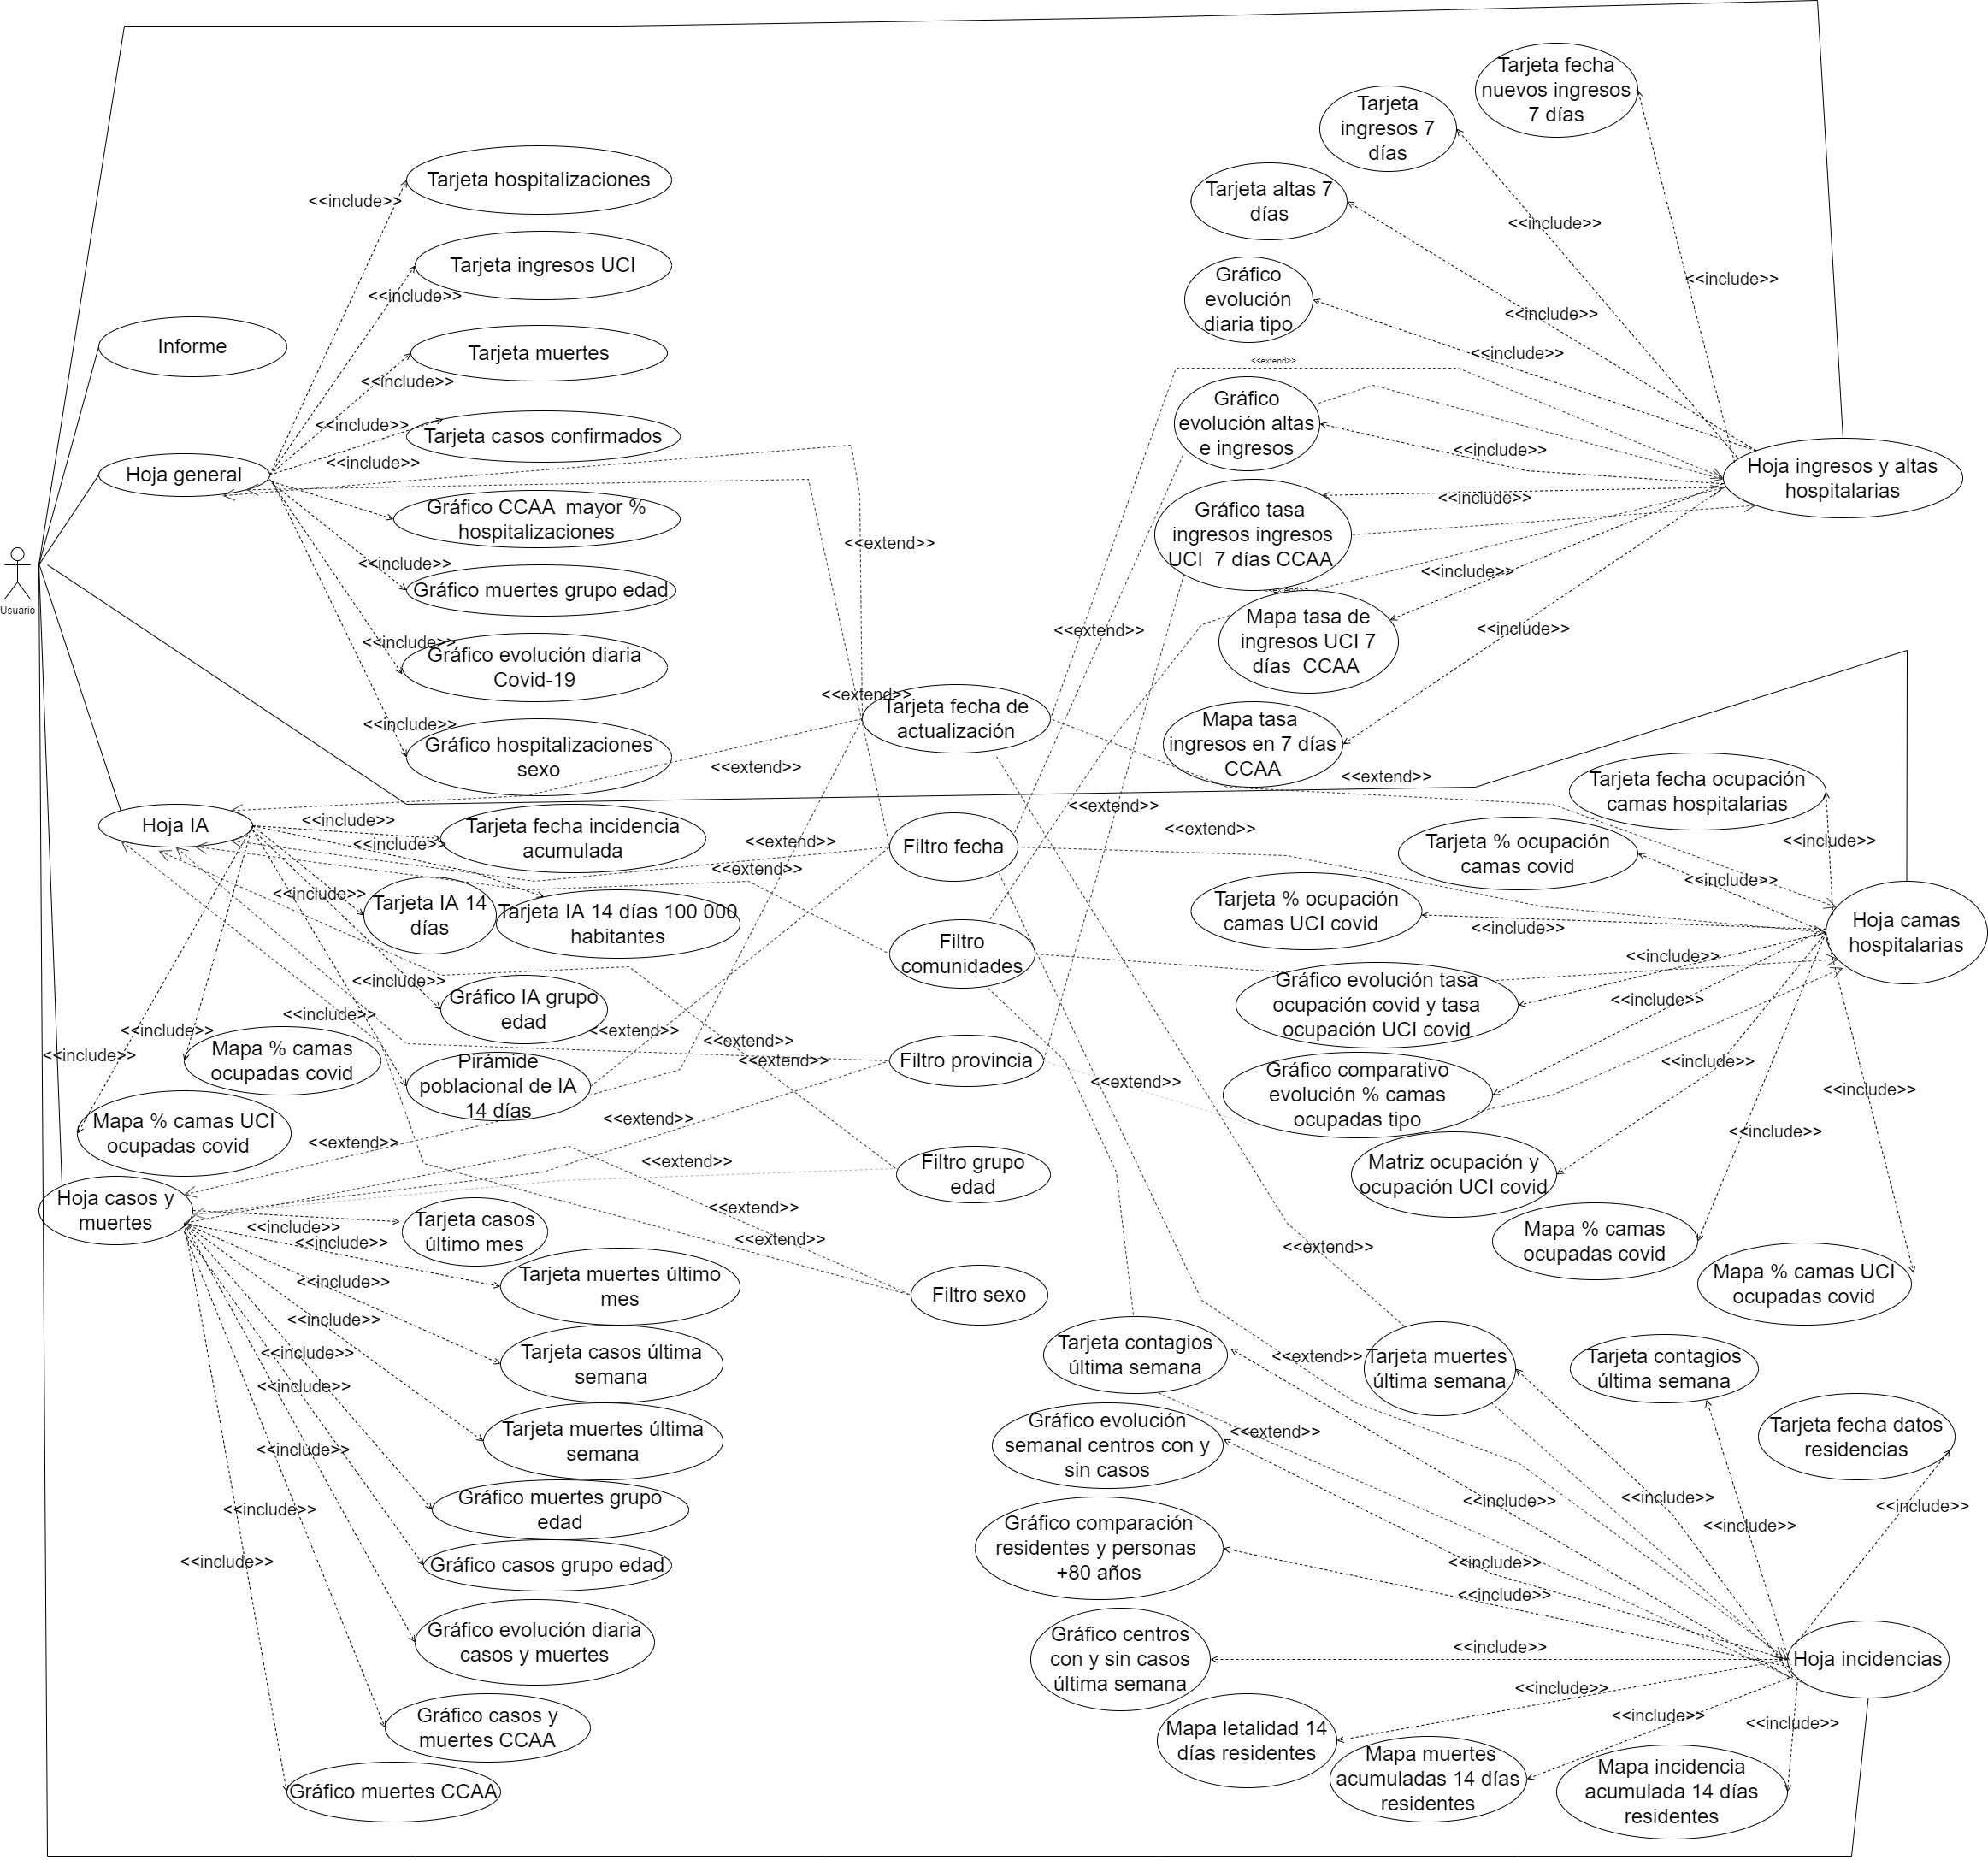
\includegraphics[scale=0.255]{img/diag2.drawio.png}
    \caption{Diagrama de casos de uso.}
\end{figure}


